

\documentclass[runningheads]{llncs}

\usepackage{graphicx}
\usepackage{times}
%\usepackage{rotate}
%\usepackage{lscape}

\begin{document}

\frontmatter          % for the preliminaries
\pagestyle{headings}  % switches on printing of running heads
\mainmatter              % start of the contributions
\title{Projet de G\'enie Logiciel\\
Rapport de Planification\\
Ann\'ee Acad\'emique 2014-2015}

\titlerunning{Rapport de planification -- \textbf{2014-2015}}

\author{Groupe num\'ero: \textbf{7}\\
Membres du groupe: \textbf{DELGRANGE FLORENT, LECOQ ALEXIS, LEMPEREUR MARTIN}}
%
\authorrunning{Groupe \textbf{7} - \textbf{BAC 2}} 

\institute{\textbf{BAC 2 INFO}\\
Facult\'e des Sciences, Universit\'e de Mons\\
\email martin.lempereur@hotmail.be \{{florent.delgrange | alexis.lecoq}\}@student.umons.ac.be
%VOUS POUVEZ UTILISER UN AUTRE ADRESSE MAIL QUE CELUI DE L'UMONS SI VOUS LE PREFERIEZ
}

\maketitle              % typeset the title of the contribution

\begin{center} \today \end{center}

Ce rapport de planification est rendu dans le cadre du cours ``Projet de G\'enie Logiciel" (dispens\'e par le Prof. \emph{Tom Mens} en ann\'ee acad\'emique 2014-2015). Le but de ce rapport est d'expliquer quels sont les objectifs
du projet, quelles sont les diff\'erentes t\^aches \`a r\'ealiser et planifier ces diff\'erentes t\^aches.


\newpage
%%%%%%%%%%%%%%%%%%%%%%%%%%%%%%%%%%%%%%%%%%%%%%%%
%%%%%%%%%%%%%%%%%%%%%%%%%%%%%%%%%%%%%%%%%%%%%%%%
\section{Introduction}\label{sec:intro}

\subsection{Objectifs}
%%Quels sont le contexte et les objectifs du projet de g\'enie logiciel?
Le travail s'inscrit dans le cadre du projet de G\'enie logiciel.
\newline Le travail consiste \`a concevoir un jeu de r\^ole dont l'unvivers est celui de l'Unviversit\'e.
\newline Nous conceverons donc une application java en d\'ecomposant la r\'ealisation  en plusieurs \'etapes cl\'es.


%%%%%%%%%%%%%%%%%%%%%%%%%%%%%%%%%%%%%%%%%%%%%%%%
\subsection{Exigences fonctionnelles}

%%\emph{Quelle est la fonctionnalit\'e demand\'e du logiciel \`a d\'evelopper?}
Nous devons impl\'ementer au moins une qu\^ete principale et secondaire de l'ann\'ee d'\'etude BAC2 et un framework permettant au joueur de r\'ealiser les diff\'erentes qu\^etes impl\'ement\'ees.

%%%%%%%%%%%%%%%%%%%%%%%%%%%%%%%%%%%%%%%%%%%%%%%%
\subsection{Exigences non-fonctionnelles}

%%\emph{Quelles sont les exigences sur la qualit\'e (p.e. portabilit\'e, fiabilit\'e, s\^uret\'e, extensibilit\'e, modularit\'e, performance  ou autre)?}

L'application doit \^etre executable sur les syst\`emes exploitation Linux, Mac et Windows.
\newline Le framework pourra supporter l'ajout de qu\^etes, de caract\`eristiques et m\^eme de classes r\'ealis\'ees par d'autres personnes ayant respect\'e l'interface commune.

%%%%%%%%%%%%%%%%%%%%%%%%%%%%%%%%%%%%%%%%%%%%%%%%
\subsection{Contraintes de temps}

Les dates importantes sont : \newline
Mardi 14 octobre 2014 : date de remise pour la phase 1 : Rapport de planification et cahier des charges.\newline
Dimanche 30 novembre 2014 : date de remise pour la phase 2 (rapport de mod\'elisation et maquette de
l'interface utilisateur) .\newline
Fin de la semaine du 10 ou d\'ebut de la semaine du 17 d\'ecembre 2014 : r\'eunions d'inspection de mod\'elisation.\newline
Jeudi 3 avril 2014 : date de remise de la phase 3 : Impl\'ementation.\newline
Les dates pour la remise de la phase 4 et de la d\'efense orale et des tests d'acceptation sont encore \'a determiner.\newline
Remarque : du lundi 22 d\'ecembre au vendredi 2 janvier, le blocus commence, il sera donc extr\^emement difficile d'\^etre productif pendant cette p\'eriode.

%%%%%%%%%%%%%%%%%%%%%%%%%%%%%%%%%%%%%%%%%%%%%%%%
\subsection{Contraintes de budget}

Aucun achat n'est pr\'evu. De plus, tous les logiciels indispensables \'a la r\'ealisation du projet sont soit gratuits, soit disponibles avec une cl\'e acad\'emique sur moodle.
\newpage
%%%%%%%%%%%%%%%%%%%%%%%%%%%%%%%%%%%%%%%%%%%%%%%%
%%%%%%%%%%%%%%%%%%%%%%%%%%%%%%%%%%%%%%%%%%%%%%%%
\section{Ressources}\label{sec:organisation}

\subsection{Les ressources humaines (personnel)}

\begin{table}[!htbp]
\begin{center}
\begin{tabular}{p{5cm}|p{5cm}|p{5cm}}
nom & r\^ole & dur\'ee \\
\hline
Florent Delgrange & d\'eveloppeur & environ 8 mois   \\
Martin Lempereur  & d\'eveloppeur & environ 8 mois  \\
Alexis Lecoq  & d\'eveloppeur & environ 8 mois  \\
Tom Mens & Titulaire du projet &   \\
Mathieu Goeminne & Enseignant &  \\
Romuald Deshayes & Assistant &   \\
\end{tabular}
\end{center}
   \caption{Ressources humaines.}
   \label{tab:RH}
\end{table}

%%%%%%%%%%%%%%%%%%%%%%%%%%%%%%%%%%%%%%%%%%%%%%%%
\subsection{Les ressources logicielles}

Les logiciels utilis\'es dans le cadre du projet sont : \newline
Gantt Project (gratuit), utilis\'e pour r\'ealiser les diagrammes de Gantt et de PERT. http://www.ganttproject.biz/ \newline
Visual Paradigm (liscence acad\'emique), utilis\'e pour r\'ealiser les diagrammes lors de la phase 2 (mod\'elisation ; diagramme de cas d'utilisation, de classe, d'\'etat, de s\'equence,...) http://www.visual-paradigm.com/ \newline
IntelliJ (liscence acad\'emique), environnement de d\'eveloppement. https://www.jetbrains.com/idea/ \newline
Eclipse (gratuit), environnement de d\'eveloppement. https://www.eclipse.org/ \newline
Git (gratuit), logiciel de gestion de versions. http://git-scm.com/ \newline
Maven (gratuit), gestion et automatisation de production des projets logiciels Java. http://maven.apache.org/ \newline
Vim (gratuit), \'editeur de texte. http://www.vim.org/. \newline
Kile (gratuit), \'editeur de texte pour les documents �crits en Latex. http://kile.sourceforge.net/ \newline
JUnit (gratuit), bien qu'il soit int\'egr\'e par d\'efaut dans Eclipse et intelliJ, il est utile de sp\'ecifier que nous utilisons ce framework pour r\'ealiser nos tests unitaires. http://junit.org/ \newline
LibGDX (gratuit), framework utilis\'e pour concevoir l'interface graphique. http://libgdx.badlogicgames.com/ \newline
Tiled Map Editor (gratuit), outil ayant pour objectif de cr�er des cartes o\'u le joueur pourra se d\'eplacer (interface graphique). http://www.mapeditor.org/ \newline

%%%%%%%%%%%%%%%%%%%%%%%%%%%%%%%%%%%%%%%%%%%%%%%%
\subsection{Les ressources mat\'erielles}

%%\emph{Quelles machines seront utilis\'ees? Pr\'excisez les caract\'�ristiques de chaque mat\'eriel: le nom, le co\^ut, le plateforme d'exploitation, le m\'empire, le processeur, le disque dur ou SSD, \ldots}

\begin{table}[!htbp]
\begin{center}
\begin{tabular}{|p{2cm}||p{2cm}|p{2cm}|p{2cm}|p{2cm}|p{2cm}|}
\hline
\textbf{Nom} & Systeme d'exploitation & Memoire & Processeur & Carte graphique & Disque dur \\
\hline\hline
Lempereur Martin &Linux&2 Go&Intel Core 2 Quad CPU Q6600 @ 2.40GHz � 4& &300 Go\\
\hline
Delgrange Florent Pc 1&Windows 8.1 pro&8 Go 1600 MHz DDR3&Intel Core i5 3470 CPU @3.20 GHZ&His Radeon R9 280X& 1To\\
\hline
Delgrange Florent Pc 2  &Mac OS X 10.9.5&4 Go 1067 MHz DDR3&2.53 GHz Intel Core 2 Duo&NVIDIA GeForce 9400M 256 Mo& \\

\hline
Lecoq Alexis& Smoby & VTech & 2Ko &  & \\
\hline
\end{tabular}
\end{center}
   \caption{Ressources materielles}
\end{table}

%%\emph{Y a-t-il des mat\'eriaux suppl\'ementaires \`a procurer? Estimer le d\'elai et les prix de ces mat\'eriaux.}

%%\emph{Les machines de d\'eveloppement seront-elles diff\'erentes des machines de d\'eploiement? Si c�est le cas,  d\'ecrivez les caract\'eristiques de chacun.}

%%\emph{Les choix effectu\'es ici devront \^etre conforme aux contraintes et exigences de la section~\ref{sec:intro}.}



%%%%%%%%%%%%%%%%%%%%%%%%%%%%%%%%%%%%%%%%%%%%%%%%
%%%%%%%%%%%%%%%%%%%%%%%%%%%%%%%%%%%%%%%%%%%%%%%%
\newpage
\section{Analyse des risques}

\subsection{Identification des risques}\label{sec:riskident}

\emph{Quels sont les risques potentiels du projet? Classifiez les risques par cat\'egorie (par exemple les risques li\'es au personnel, au produit, au projet; d'autres classifications sont permises).  Distinguez les risques g\'en\'eriques (au moins 4), applicables \`a tout projet (informatique), des risques sp\'ecifiques (au moins 4) pour votre propre projet. Donnez une description textuelle de chaque risque.}

\emph{Prioritisez les risques selon leur importance, en fonction de leur probabilit\'e et s\'ev\'erit\'e. Vous devez justifier la probabilit\'e et s\'ev\'erit\'e de chaque risque.
Si vous le souhaitez, vous pouvez utiliser une table pour r\'esumer les risques retenus, comme par exemple la Table~\ref{tab:risques}.}


\begin{table}[!htbp]
\begin{center}
\begin{tabular}{|p{3cm}||c|c|}
\hline
\textbf{Risque} & Probabilit\'e & S\'ev\'erit\'e\\
\hline\hline
risque 1 & basse &  non significative \\
\hline
risque 2 & \Large{haute} &  tol\'erable \\
\hline
risque 3 & \large{mod\'er\'ee} & \large{s\'erieuse} \\
\hline
risque 4 & basse & \Large{catastrophique} \\
\hline
\end{tabular}
\end{center}
   \caption{Analyse des risques.}
   \label{tab:risques}
\end{table}

%\`A titre d'information, voici quelques exemples de risques souvent rencontr\'es dans un projet informatique:
%\begin{itemize}
%\item difficult\'es techniques impr\'evues (probl\`eme de versions, probl\`eme de compatibilit\'e, mat\'eriel ou logiciel d\'efectueux, perte de donn\'ees, ...)
%\item difficult\'e de compr\'ehension (documentation non disponible en fran\c{c}ais, documentation absent, sujet ou domaine complex et difficile \`a ma\^itriser, ...)
%\item probl\`eme de ressources (mat\'erial non disponible, indisponibilit\'e du directeur ou autres personnes impliqu\'ees dans le travail, manque de communication)
%\item probl\`eme d'horaire (manque de temps, horaire de cours inflexible, maladie, ...)
%\item probl\`eme du produit final (incompl\`ete, peu performant, instable, d\'efectueux, manque de documentation, difficile \`a utiliser ou maintenir, probl\`eme de fiabilit\'e ou s\'ecurit\'e, ...)
%\end{itemize}
%
%Cette liste \textbf{n'est pas exhaustive} et peut varier selon le contexte du travail. Ce qui est important se sont les risques qui sont vraiment sp\'ecifiques \`a votre projet.

%%%%%%%%%%%%%%%%%%%%%%%%%%%%%%%%%%%%%%%%%%%%%%%%
\subsection{Gestion des risques}\label{sec:riskmanagement}

Pour chaque risque que vous avez retenu dans la section \ref{sec:riskident} (en fonction de son importance), expliquez comment vous comptez 
\begin{enumerate}
\item \'eviter que le risque se produira
\item v\'erifier si le risque s'est produit
\item r\'esoudre ou r\'eduire l'ampleur du risque quand il s'est produit
\end{enumerate}

%%%%%%%%%%%%%%%%%%%%%%%%%%%%%%%%%%%%%%%%%%%%%%%%
%%%%%%%%%%%%%%%%%%%%%%%%%%%%%%%%%%%%%%%%%%%%%%%%
\newpage
\section{R\'epartition du travail}

\subsection{Work Breakdown Structure}

%%\emph{Mettez la r\'epartition des t\^aches et sous-t\^aches, ou l'horaire du projet ici. Indiquez \'egalement qui fait quelle t\^ache.
%%Pour ce faire, vous pouvez inclure une figure ici (extrait d'un outil de planification), ou vous pouvez mettre les informations dans un tableau de t\^aches, comme par exemple Table~\ref{tab:WBS}.}

%\begin{table}[htbp]
%\begin{center}
%\begin{tabular}{|r|p{4cm}||p{2cm}|p{2cm}|c|c|c|}
%\hline
%\textbf{ID} & T\^ache & Dates & Responsable & \% travail & Autre remarques\\
%%\hline\hline
%T1 & \'Diagramme de cas d'utilisation & 14  & ... l'\'etudiant ... & 100\% &\\
%%\hline
%%\hline
%%T2 & description t\^ache 2 & & &  & \\
%%\hline
%%T3 & description t\^ache 3 & & & &\\
%%\hline
%%\end{tabular}
%%\end{center}
 %%  \caption{Tableau des t\^aches.}
  %% \label{tab:WBS}
%%\end{table}
\begin{figure}[!htb]
\begin{center}
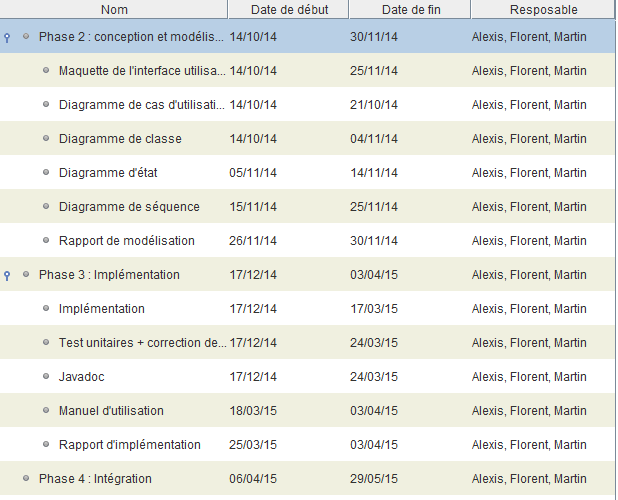
\includegraphics[width = \textwidth]{repartition.PNG}
\caption{Tableau des t\^aches.}\label{fig:repartition}
\end{center}
\end{figure}
Remarque : la r\'epartition du travail ainsi que les dates ne sont pas d\'efinitives.

%%%%%%%%%%%%%%%%%%%%%%%%%%%%%%%%%%%%%%%%%%%%%%%%
\subsection{Etapes cl\'es }

%%\emph{Quels sont les \'etapes cl\'es (milestones)? Quelles sont les livrables (si pr\'esent) pour chaque \'etape cl\'e? Donnez une description du contenu de chaque livrable.
%%Vous pouvez utiliser un tableau d'\'etapes cl\'es pour repr\'esenter une partie de l'information requise, comme par exemple Table~\ref{tab:TEC}.}

\begin{table}[htbp]
\begin{center}
\begin{tabular}{|p{2.5cm}||p{6cm}|p{3cm}|}
\hline
Date & \'etape cl\'e & Livrables\\
\hline\hline
14 octobre 2014 & Date de remise pour la phase 1 & Rapport de planification et cahier des charges\\
\hline
30 novembre 2014 & Date de remise pour la phase 2 & Rapport de mod\'elisation et maquette de
l'interface utilisateur. \\
\hline
10 au 17 d\'ecembre 2014 & R\'eunions d'inspection de mod\'elisation &  \\
\hline
3 avril 2014 & Date de remise de la phase 3 & Impl\'ementation \\
\hline
? & Date de remise de la phase 4 & Int\'egration \\
\hline
? & D\'efense orale, tests d'acceptation par les enseignants & \\
\hline
\end{tabular}
\end{center}
   \caption{Tableau d'\'etapes cl\'es.}
   \label{tab:TEC}
\end{table}

%%%%%%%%%%%%%%%%%%%%%%%%%%%%%%%%%%%%%%%%%%%%%%%%
%%%%%%%%%%%%%%%%%%%%%%%%%%%%%%%%%%%%%%%%%%%%%%%%
\newpage
\section{Ordonnancement}

\subsection{Diagramme GANTT}

%%\emph{Vous devriez inclure et discuter ici un ou plusieurs diagrammes de GANTT, comme ceux montr\'es dans les Figures~\ref{fig:GANTT} et~\ref{fig:GANTT2}. \`A vous de choisir comment g\'en\'erer le(s) diagramme(s). Pr\'ecisez le ou les outils utilis\'es pour la cr\'eation de chaque diagramme.}

\begin{figure}[!htb]
\begin{center}
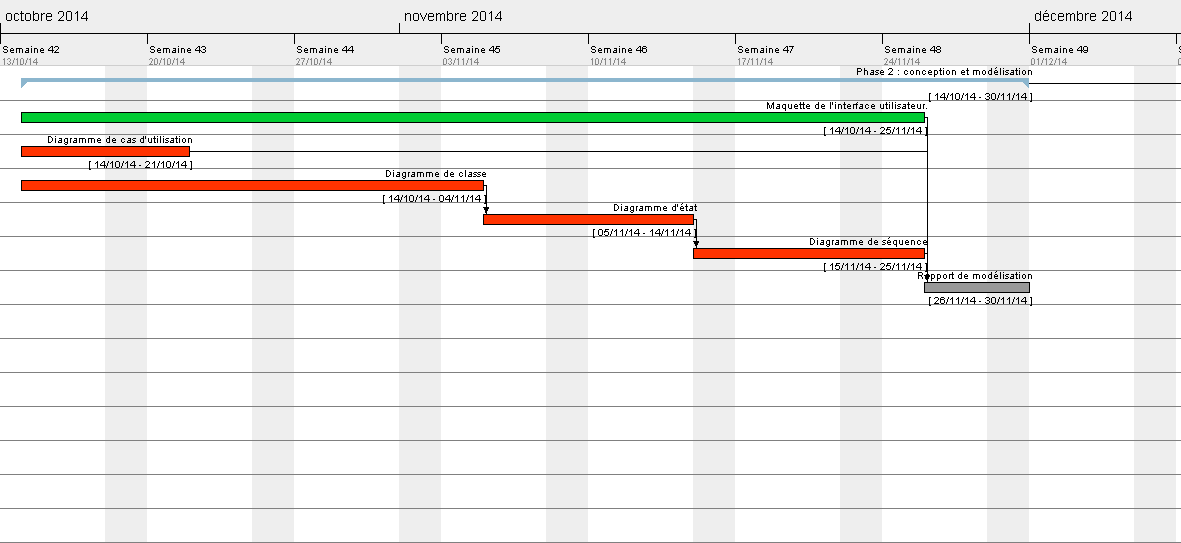
\includegraphics[width=\textwidth]{Gantt1.png}
  \caption{Diagramme Gantt de la phase 1.}\label{fig:Phase 1}
\end{center}
\end{figure}

\begin{figure}[!htb]
\begin{center}
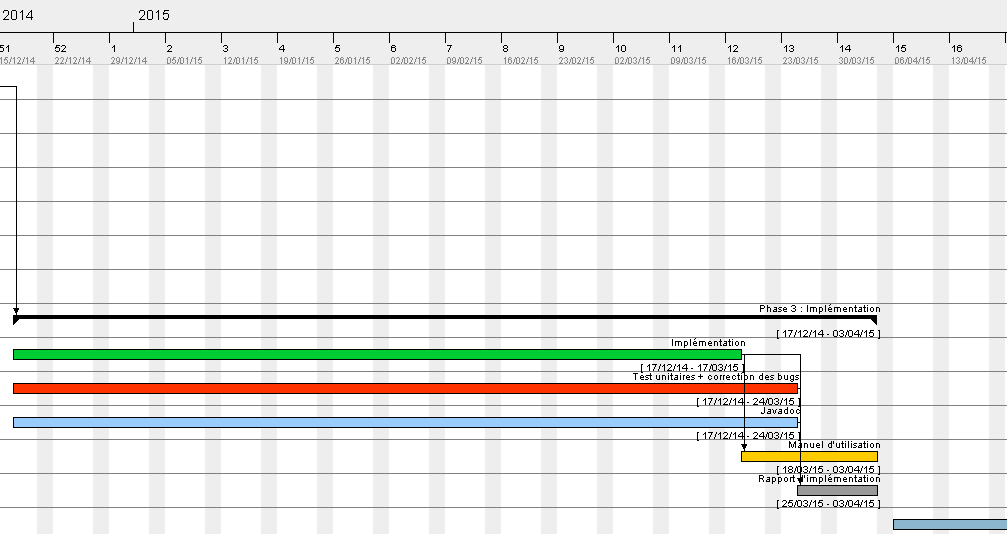
\includegraphics[width=\textwidth]{Gantt2.png}
  \caption{Diagramme Gantt de la phase 2.}\label{fig:Phase 2}
\end{center}
\end{figure}

%%\emph{N'oubliez pas d'indiquer, sur le diagramme, les \'etapes cl\'es et les d\'ependances entre les t\^aches. Si l'outil que vous avez utilis\'e ne permet pas de faire cela, vous pouvez mettre cette information dans une table s\'epar\'ee, comme par exemple Table~\ref{tab:GANTT}.}

%\begin{table}[htbp]
%\begin{center}
%\begin{tabular}{|p{2cm}||c|c||c|}
%\hline
%\textbf{T\^ache} & Pr\'edecesseurs \\
%\hline\hline
%id tache 1 &   \\
%\hline
%id tache 2 &  \\
%\hline
%id tache 3 & \\
%\hline
%�\end{tabular}
%\end{center}
 %  \caption{D\'ependances entre les t\^aches.}
 %  \label{tab:GANTT}
%\end{table}

%%%%%%%%%%%%%%%%%%%%%%%%%%%%%%%%%%%%%%%%%%%%%%%%
\subsection{Diagramme PERT}

%%\emph{Vous devriez inclure et discuter ici un ou plusieurs diagrammes  PERT, comme ceux montr\'es dans les Figure~\ref{fig:PERT} et Figure~\ref{fig:PERT2}. \`A vous de choisir comment g\'en\'erer ce diagramme. Pr\'ecisez le ou les outils utilis\'es pour la cr\'eation de chaque diagramme.}

\begin{figure}[!htb]
\begin{center}
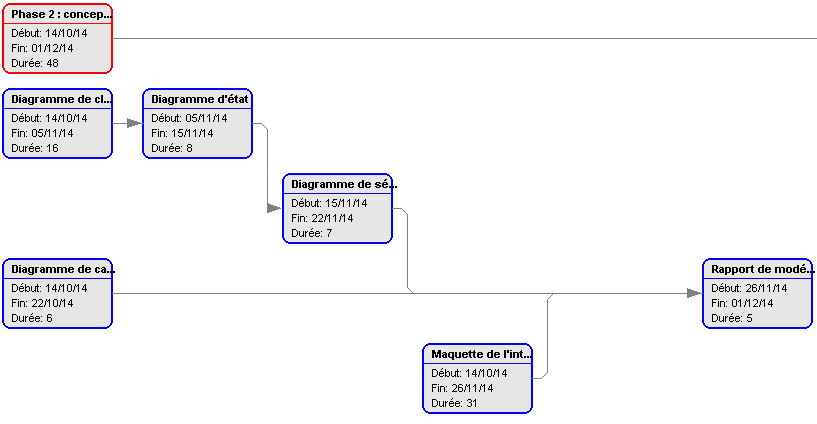
\includegraphics[width=\textwidth]{PERT1.PNG}
  \caption{Diagramme PERT de la phase 1.}\label{fig:PERT1}
\end{center}
\end{figure}

\begin{figure}[!htb]

\begin{center}
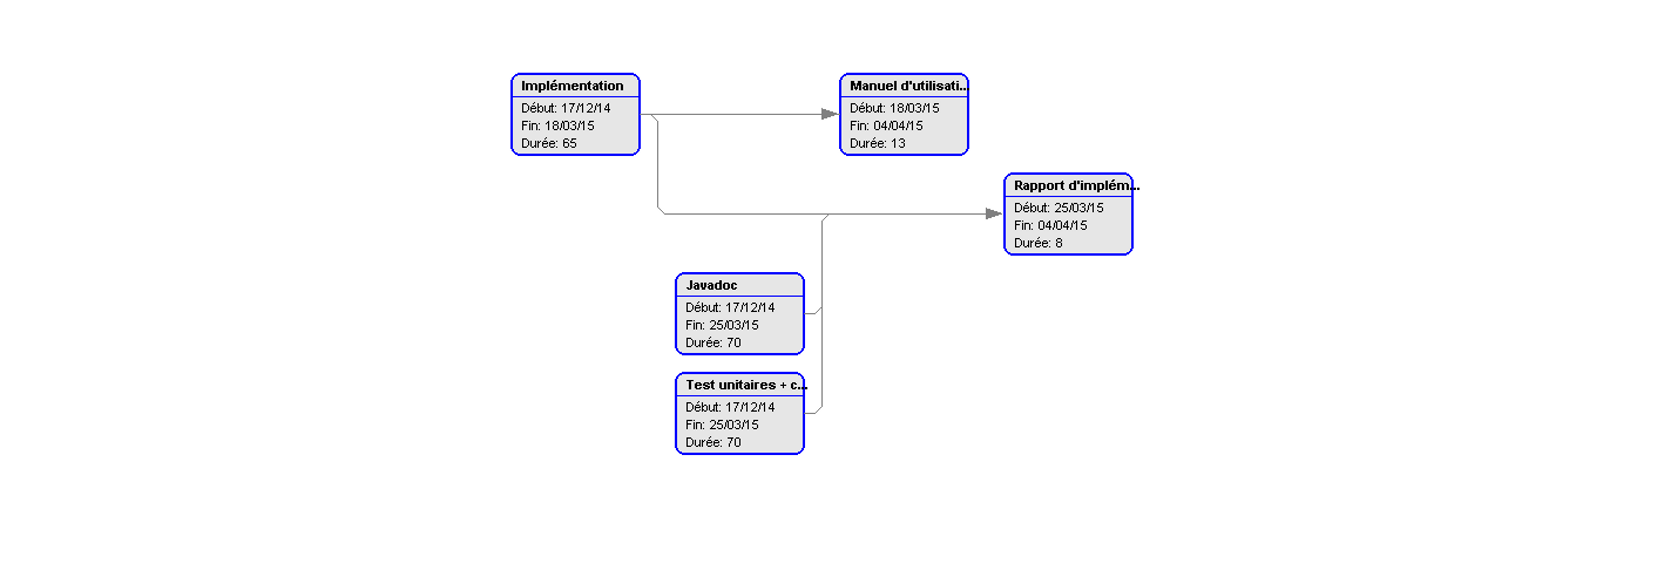
\includegraphics[width=\textwidth]{PERT4.PNG}
  \caption{Diagramme PERT de la phase 2.}\label{fig:PERT2}
\end{center}
\end{figure}

%%Si l'outil que vous avez utilis\'e pour g\'en\'erer le diagramme PERT le permet, vous devriez indiquer dans le diagramme, pour chaque t\^ache, la dur\'ee, l'effort (en personne/mois), le temps "Earliest Start (ES)", le temps "Latest Start (LS)", le temps l\^ache (\emph{Slack Time (ST)}), et le \emph{Free Float (FF)}. Le diagramme doit \'egalement montrer o\`u se trouve le(s) chemin(s) critique(s).

%%Si l'outil que vous avez utilis\'e ne le permet pas vous devriez mettre ces informations dans une table s\'epar\'ee, comme par exemple la Table~\ref{tab:PERT}.

\begin{table}[htbp]
\begin{center}
\begin{tabular}{|p{4cm}||c|c|c|c|c|c|}
\hline
\textbf{T\^ache} & Dur\'ee (jours) & Effort & Earliest Start & Latest Start & Slack Time & Free Float\\
\hline\hline
Diagramme de classes & 16 & Eleve & 14/10/14 &  14/10/14  & 0 & 0 \\
\hline
Diagramme de cas d'utilisation & 6 & Moyen & 14/10/14 & 24/11/14 & 41 & 41 \\
\hline
Diagramme d'�tats & 8 & Moyen & 05/11/14 &  05/11/14 & 0 & 0 \\
\hline
Diagramme de s�quences & 7 & Moyen & 15/11/14 & 15/11/14 & 0 & 0 \\
\hline
Maquette de l'interface & 31 & Eleve & 14/10/14 & 14/10/14 & 0 & 0 \\
\hline
Rapport de mo�d�lisation & 5 & Moyen & 26/11/14 & 26/11/14 & 0 & 0 \\
\hline
Implementation & 65 & Eleve & 17/12/14 & 17/12/14 & 0 & 0 \\
\hline
Javadoc &  70 & Faible & 17/12/14 & 17/12/14 & 0 & 0 \\
\hline
Tests unitaires & 70 & Eleve & 17/12/14 & 17/12/14 & 0 & 0 \\
\hline
Manuel d'utilisation & 13 & Faible & 18/03/15 & 18/03/15 & 0 & 0 \\
\hline
Rapport d'implementation & 8 & Moyen & 25/03/15 & 25/03/15 & 0 & 0 \\
\hline
\end{tabular}
\end{center}
   \caption{Informations temporelles importantes sur les t\^aches.}
   \label{tab:PERT}
\end{table}

%%%%%%%%%%%%%%%%%%%%%%%%%%%%%%%%%%%%%%%%%%%%%%%%
\subsection{Analyse de l'ordonnancement}

\emph{Analysez les diagrammes en calculant le chemin critique, les temps l\^aches (marge totale) et la marge libre (free float), tout en v\'erifiant que vous avez fait un bon choix. (Si non, vous devriez modifier votre ordonnancement afin de l'optimiser...)
Justifiez votre d\'ecision.}

%%%%%%%%%%%%%%%%%%%%%%%%%%%%%%%%%%%%%%%%%%%%%%%%
\subsection{Surveillance}

\emph{Expliquez comment vous comptez surveiller les retards \'eventuels du projet quand il est en cours de route. Quelle proc\'edure allez vous suivre pour d\'etecter et \'eviter ces retards? Qu'allez vous faire quand un retard se manifeste?}

\emph{Expliquez \'�galement comment vous comptez surveiller les risques.}

\bibliographystyle{splncs}
\bibliography{biblio}

\end{document}
